\documentclass[11pt,a4paper]{article}
\usepackage{fontspec}
\setmainfont{texgyretermes}[Extension=.otf,UprightFont=*-regular,BoldFont=*-bold,ItalicFont=*-italic,BoldItalicFont=*-bolditalic]
\setsansfont{texgyreheros}[Extension=.otf,UprightFont=*-regular,BoldFont=*-bold,ItalicFont=*-italic,BoldItalicFont=*-bolditalic]
\setmonofont{lmmono10}[Extension=.otf,UprightFont=*-regular]
\usepackage[a4paper,margin=2.2cm]{geometry}
\usepackage{graphicx,booktabs,tabularx,array,amsmath,amssymb,float,enumitem,xcolor}
\usepackage[font=small,labelfont=bf]{caption}
\usepackage[most]{tcolorbox}
\usepackage[colorlinks=true,linkcolor=teal!60!black,urlcolor=teal!60!black]{hyperref}
\usepackage{titlesec}

\definecolor{acc}{HTML}{2A78D6}
\titleformat{\section}{\Large\sffamily\bfseries\color{acc!75!black}}{\thesection}{0.6em}{}
\titleformat{\subsection}{\large\sffamily\bfseries}{\thesubsection}{0.5em}{}
\titlespacing*{\section}{0pt}{12pt}{5pt}
\titlespacing*{\subsection}{0pt}{8pt}{3pt}
\setlist{itemsep=2pt,topsep=3pt}
\renewcommand{\arraystretch}{1.18}
\newtcolorbox{ghichu}[1][Điểm cần nhớ]{colback=acc!5,colframe=acc!70!black,fonttitle=\sffamily\bfseries,title=#1,
  boxrule=0.6pt,arc=2pt,left=6pt,right=6pt,top=4pt,bottom=4pt}
\captionsetup{justification=raggedright,singlelinecheck=false}
\graphicspath{{figs/}}
\renewcommand{\figurename}{Hình}
\renewcommand{\tablename}{Bảng}
\setcounter{topnumber}{3}\setcounter{totalnumber}{4}\renewcommand{\topfraction}{0.9}\renewcommand{\textfraction}{0.1}\renewcommand{\floatpagefraction}{0.8}
\newcommand{\Avg}{\mathrm{Avg}}


\begin{document}

\begin{center}
{\sffamily\bfseries\LARGE UPAR Challenge 2027 \textendash{} Track 1\\[3pt]
\Large Nhận dạng đặc điểm người đi bộ trên camera chưa từng thấy}\\[8pt]
{\large Báo cáo kết quả, viết cho người đọc chưa quen với học máy}\\[5pt]
{\small Cập nhật ngày 02/10/2026 \quad Tài khoản Codabench \texttt{tannguyenbmt47}}
\end{center}

\begin{ghichu}[Tóm tắt]
\begin{itemize}[leftmargin=1.2em]
\item Cuộc thi yêu cầu một chương trình nhìn ảnh một người đi bộ và cho biết 40 đặc điểm của người đó, như tuổi, giới tính, màu áo, màu quần và phụ kiện. Chương trình được chấm trên ảnh từ những camera mà nó chưa từng thấy khi học.
\item Bài nộp tốt nhất của đội đạt 0.7857 điểm trên tập chấm ẩn của ban tổ chức, cao hơn 0.0082 điểm so với bài tốt nhất trước đó (0.7775).
\item Mức tăng này đến từ việc dùng một mô hình lớn hơn. Khoảng 35 thay đổi nhỏ khác ở cách học và cách ra quyết định đều không giúp được.
\item Giới hạn lớn nhất của cuộc thi là thời gian chạy. Server chấm bài chỉ có 6 luồng xử lý của CPU và cho tối đa 60 phút, nên mô hình lớn phải chạy trên ảnh nhỏ hơn để kịp giờ.
\end{itemize}
\end{ghichu}

\section{Bài toán}

\subsection{Chương trình phải làm gì}

Các hệ thống camera giám sát thường cần tìm người theo mô tả, ví dụ ``một phụ nữ mặc áo hồng, váy đen''. Muốn vậy, máy tính phải tự nhìn ảnh và nói ra các đặc điểm của người trong ảnh. Bài toán này gọi là pedestrian attribute recognition (tạm dịch: nhận dạng thuộc tính người đi bộ).

Mỗi ảnh đầu vào là một khung hình chữ nhật đứng, cắt sẵn quanh một người. Với mỗi ảnh, chương trình phải trả về 40 con số từ 0 đến 1. Mỗi con số là xác suất mà người trong ảnh có một attribute (tạm dịch: thuộc tính) cụ thể, ví dụ ``là nữ'', ``mặc áo đỏ'' hay ``đeo ba lô''. Hình~\ref{fig:io} cho ba ví dụ thật. Cột xanh là những thuộc tính người đó thật sự có, cột xám là những thuộc tính không có, và chiều cao cột là xác suất mà chương trình đưa ra.

\begin{figure}[H]
\centering
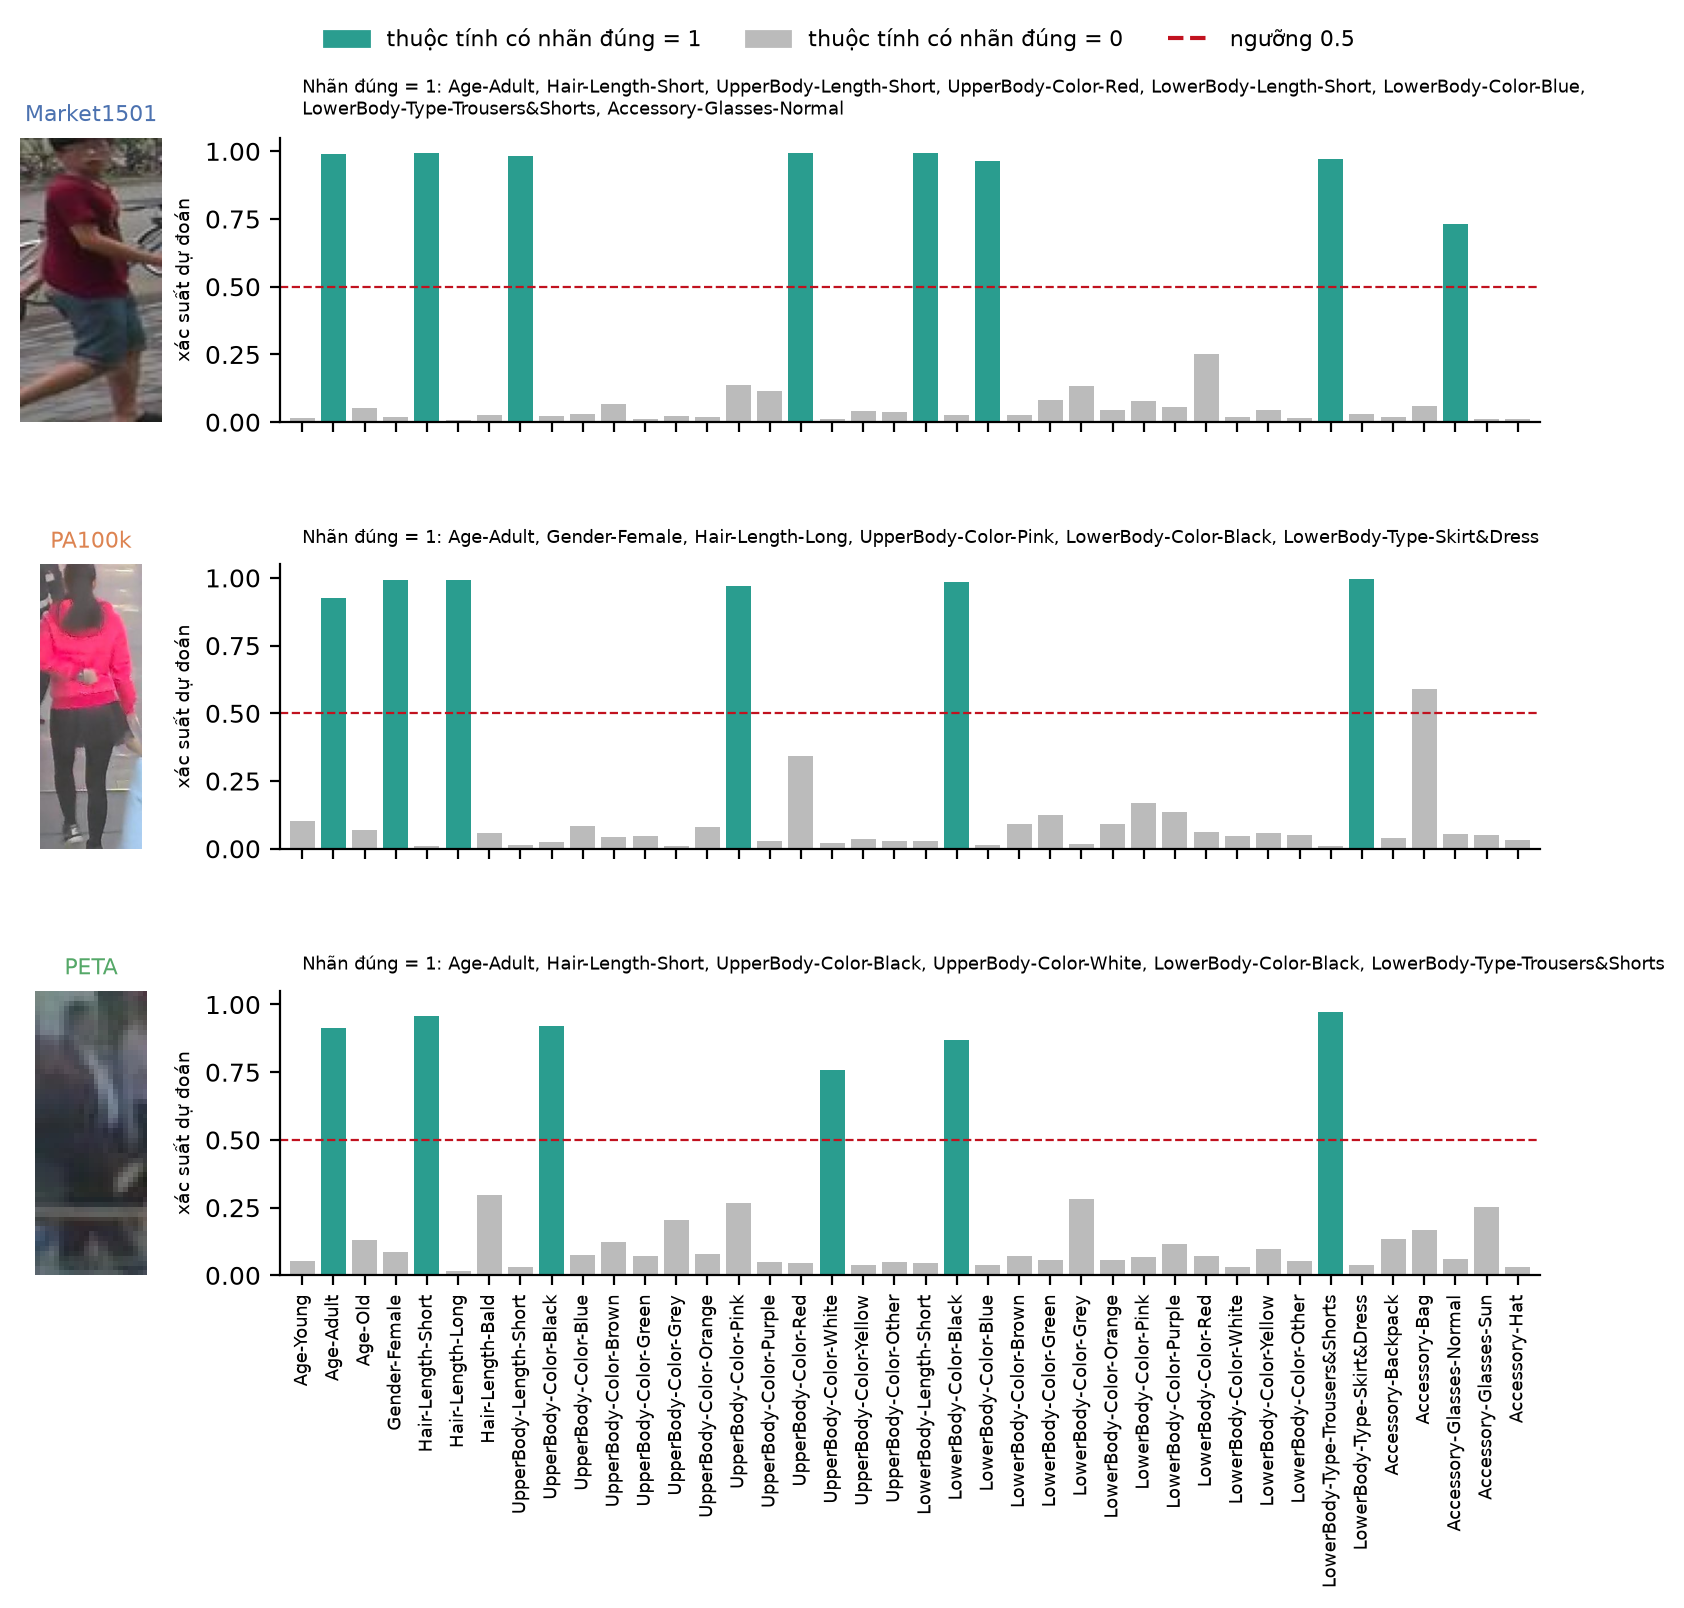
\includegraphics[width=0.92\linewidth]{io_example.png}
\caption{Ba ảnh thật và 40 xác suất mà chương trình dự đoán cho mỗi ảnh. Đường đỏ là ngưỡng 0.5. Cột cao hơn ngưỡng nghĩa là chương trình trả lời có.}
\label{fig:io}
\end{figure}

Hệ thống chấm điểm biến xác suất thành câu trả lời có hoặc không bằng một threshold (tạm dịch: ngưỡng) cố định là 0.5. Xác suất trên 0.5 là có, dưới 0.5 là không. Ở ảnh thứ hai của Hình~\ref{fig:io}, chương trình trả lời đúng cả 6 thuộc tính người phụ nữ có. Tuy nhiên nó cho thuộc tính ``mang túi xách'' xác suất 0.59, vượt ngưỡng, nên trả lời có, trong khi người này không mang túi. Đây là một lỗi.

Bốn mươi thuộc tính chia thành vài nhóm, gồm tuổi (trẻ, trưởng thành, già), giới tính, tóc (ngắn, dài, hói), áo (ngắn tay và 12 màu), quần (ngắn, 12 màu, quần hay váy) và 5 loại phụ kiện. Riêng màu sắc đã chiếm 24 trong 40 thuộc tính. Trong nhiều nhóm, mỗi người chỉ có đúng một lựa chọn, ví dụ một độ tuổi hoặc một màu quần.

\subsection{Dữ liệu học và vì sao bài toán khó}

Chương trình học từ khoảng 131.000 ảnh đã được con người gán nhãn, lấy từ ba dataset (tạm dịch: bộ dữ liệu) công khai là Market1501, PA100k và PETA (Hình~\ref{fig:samples}). Mỗi bộ được chụp bằng những camera khác nhau, ở những nơi khác nhau. Market1501 chụp trước một siêu thị, ảnh nhỏ và khá giống nhau. PA100k chụp ngoài trời từ gần 600 camera và chiếm 81\% số ảnh. PETA gộp từ mười bộ nhỏ hơn, nhiều ảnh mờ hoặc ám màu.

\begin{figure}[H]
\centering
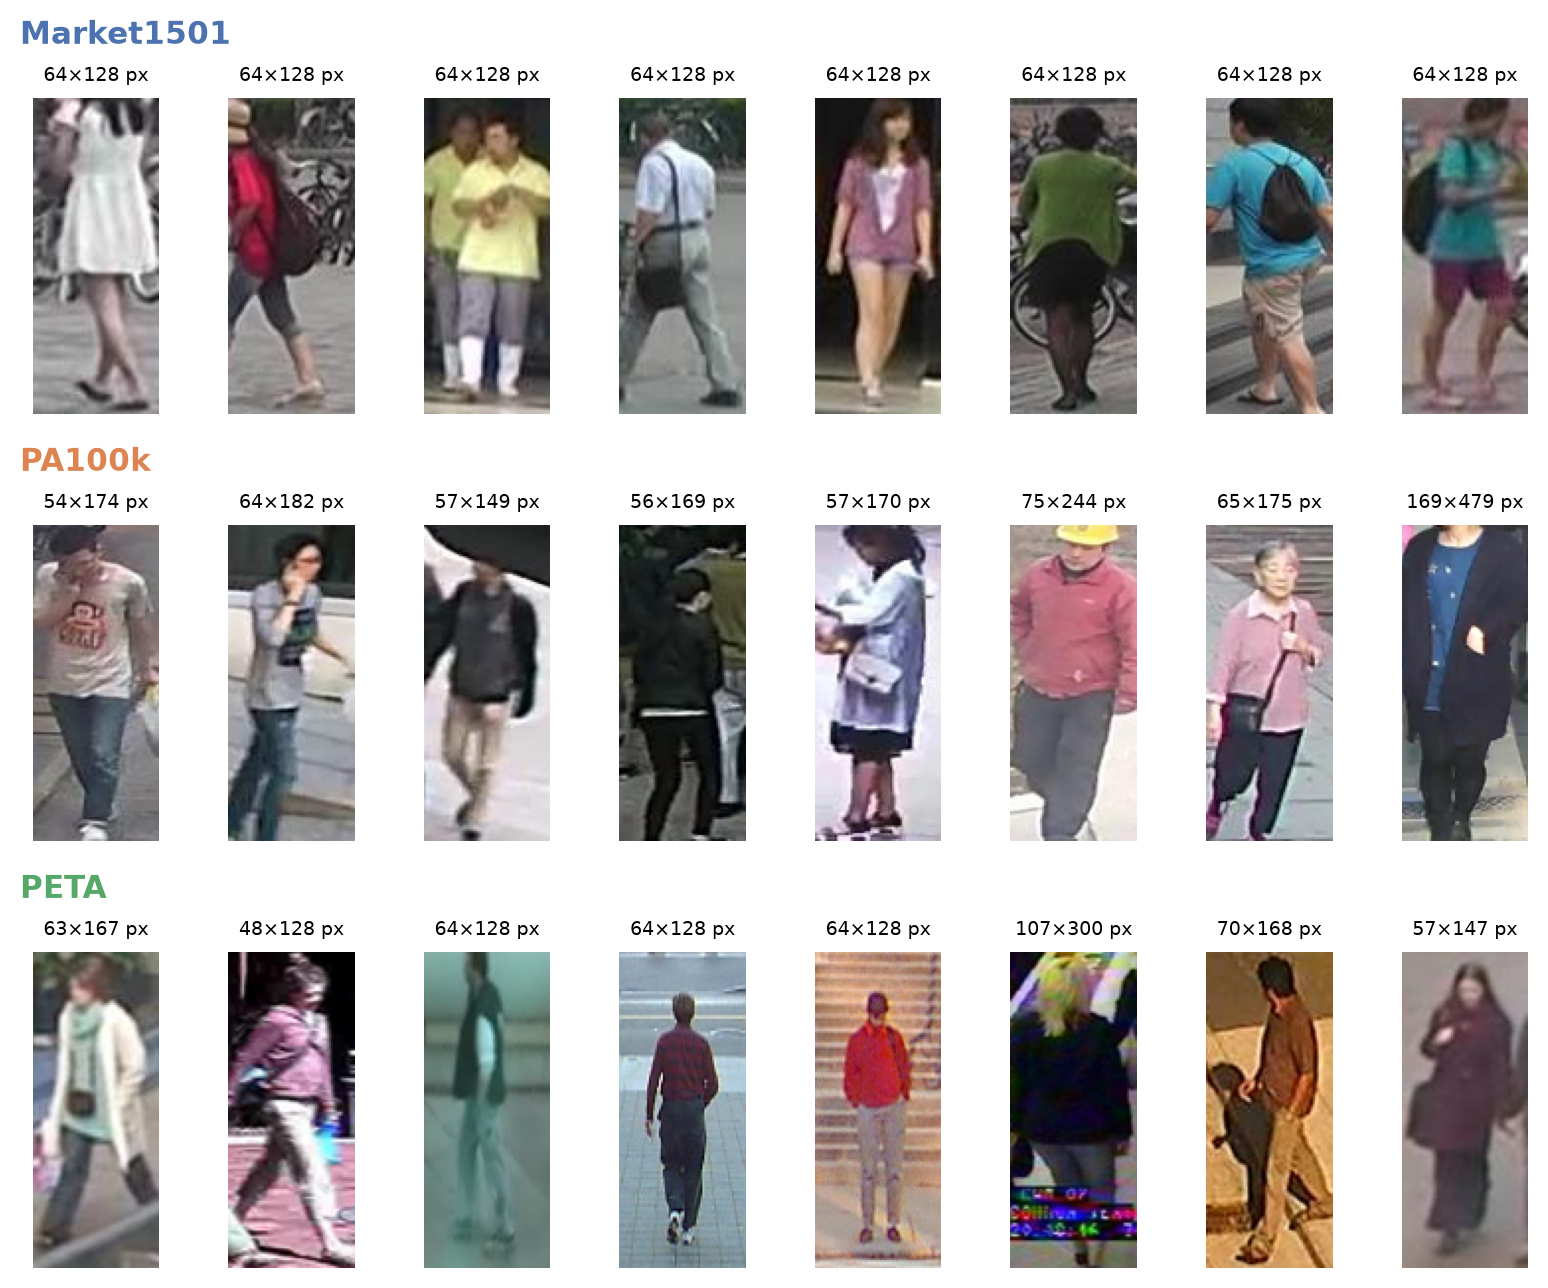
\includegraphics[width=0.78\linewidth]{samples.png}
\caption{Ảnh mẫu của ba bộ dữ liệu dùng để học, với kích thước gốc ghi phía trên mỗi ảnh. Mỗi bộ có độ phân giải, góc chụp và màu sắc riêng.}
\label{fig:samples}
\end{figure}

Điểm khó nhất là ban tổ chức chấm bài trên một bộ ảnh từ camera khác hẳn ba bộ trên, và không công bố bộ ảnh đó. Hiện tượng dữ liệu lúc chấm khác dữ liệu lúc học gọi là domain shift (tạm dịch: lệch miền dữ liệu). Mỗi bộ dữ liệu là một domain (tạm dịch: miền dữ liệu) riêng, với ánh sáng, độ nét và góc chụp riêng.

Các miền còn khác nhau ở cách con người gán nhãn. Tỉ lệ người già là 1\% trong Market1501 nhưng hơn 6\% trong PETA. Người gán nhãn PETA đôi khi ghi hai màu cho một chiếc áo, còn hai bộ kia luôn ghi đúng một màu. Một chương trình học thuộc thói quen của ba bộ cũ sẽ mắc lỗi khi gặp bộ mới có thói quen khác. Thực tế, chương trình đầu tiên của đội đạt 0.885 điểm trên ảnh cùng loại với ảnh đã học, nhưng chỉ 0.777 trên tập chấm của ban tổ chức.

\subsection{Giới hạn khi chạy bài}

Đội không nộp câu trả lời mà nộp chính chương trình. Server của ban tổ chức chạy chương trình trên 29.248 ảnh, chỉ bằng 6 luồng xử lý của CPU (tạm dịch: bộ xử lý trung tâm), không có GPU (tạm dịch: card đồ hoạ dùng để tính nhanh) và không có Internet. Toàn bộ phải xong trong 60 phút, nên trung bình mỗi ảnh chỉ được xử lý trong khoảng 0,11 giây. Mô hình càng lớn thì càng chính xác nhưng càng chậm, nên giới hạn thời gian quyết định đội được dùng mô hình lớn đến đâu. Mỗi ngày đội được nộp ba lần, và bảng xếp hạng chỉ giữ bài nộp gần nhất.

\section{Cách chấm điểm}
\label{sec:metrics}

\subsection{Hai cách đếm lỗi}

Ban tổ chức đếm lỗi theo hai cách rồi gộp lại. Cách thứ nhất xét từng thuộc tính. Với thuộc tính ``người già'', ta xem chương trình nhận ra bao nhiêu phần trăm số người già thật, và nhận đúng bao nhiêu phần trăm số người không già, rồi lấy trung bình hai tỉ lệ đó. Làm như vậy cho cả 40 thuộc tính rồi lấy trung bình, ta được mA (mean accuracy, tạm dịch: độ chính xác trung bình theo thuộc tính).
\begin{equation}
\mathrm{mA}=\frac{1}{40}\sum_{k=1}^{40}\frac12\Big(\underbrace{\tfrac{\text{số người có thuộc tính }k\text{ được nhận ra}}{\text{số người có thuộc tính }k}}_{\text{tỉ lệ nhận ra}}+\underbrace{\tfrac{\text{số người không có }k\text{ được trả lời không}}{\text{số người không có }k}}_{\text{tỉ lệ không báo nhầm}}\Big).
\end{equation}
Cách đếm này coi mọi thuộc tính quan trọng như nhau. Người già chỉ chiếm 1\% đến 6\% số ảnh, nhưng thuộc tính ``người già'' vẫn có trọng số bằng thuộc tính ``mặc quần dài'' vốn gặp ở phần lớn ảnh. Một chương trình lười, luôn trả lời không cho ``người già'', đúng ở 99\% số ảnh nhưng chỉ được 0.5 điểm cho thuộc tính này, vì nó không nhận ra người già nào.

Cách thứ hai xét từng ảnh. Với mỗi ảnh, ta so tập thuộc tính chương trình trả lời có với tập thuộc tính người đó thật sự có, bằng chỉ số F1 (tạm dịch: điểm cân bằng giữa độ chính xác và độ đầy đủ).
\begin{equation}
\mathrm{F1}_{\text{ảnh}}=\frac{2\times\text{số thuộc tính trả lời có và đúng}}{\text{số thuộc tính trả lời có}+\text{số thuộc tính thật sự có}} .
\end{equation}
Trung bình F1 trên mọi ảnh là Instance F1 (tạm dịch: F1 theo từng ảnh). Ở ví dụ người phụ nữ áo hồng, chương trình trả lời có 7 thuộc tính, trong đó 6 đúng, và người đó có 6 thuộc tính. F1 của ảnh này là $2\times6/(7+6)\approx0.92$. Nếu không có lỗi túi xách, F1 sẽ là 1.

Điểm xếp hạng cuối cùng là Challenge\_Avg (tạm dịch: điểm tổng của cuộc thi). Đây là harmonic mean (tạm dịch: trung bình điều hoà) của mA và Instance F1, bằng $2\times\mathrm{mA}\times\mathrm{F1}/(\mathrm{mA}+\mathrm{F1})$. Trung bình điều hoà luôn gần với số nhỏ hơn. Vì vậy một chương trình rất giỏi ở một cách đếm nhưng kém ở cách kia vẫn bị điểm thấp.

\subsection{Hai cách đếm kéo về hai phía}

Hai cách đếm này muốn những điều ngược nhau. mA thưởng cho việc dám trả lời có ở thuộc tính hiếm, vì bỏ sót một người già bị phạt nặng. Instance F1 lại phạt mỗi câu trả lời có bị sai. Mỗi người chỉ có khoảng 7 thuộc tính thật trên 40, nên một câu trả lời thừa làm F1 của ảnh đó giảm từ 1 xuống khoảng 0.93.

Đội điều chỉnh sự cân bằng này bằng cách dời ngưỡng của từng thuộc tính, gọi là offset (tạm dịch: độ dời ngưỡng). Một offset dương giúp thuộc tính dễ được trả lời có hơn. Offset được tính tự động trên ảnh của ba bộ dữ liệu cũ rồi giảm bớt theo một hệ số, vì miền mới có thể khác miền cũ. Hình~\ref{fig:metric} cho thấy khi tăng hệ số này từ 0 lên 1, mA tăng từ 0.766 lên 0.802 còn Instance F1 giảm từ 0.808 xuống 0.790. Điểm tổng tăng nhanh lúc đầu rồi gần như không đổi trong khoảng 0.6 đến 1. Đội dùng hệ số 0.6.

\begin{figure}[H]
\centering
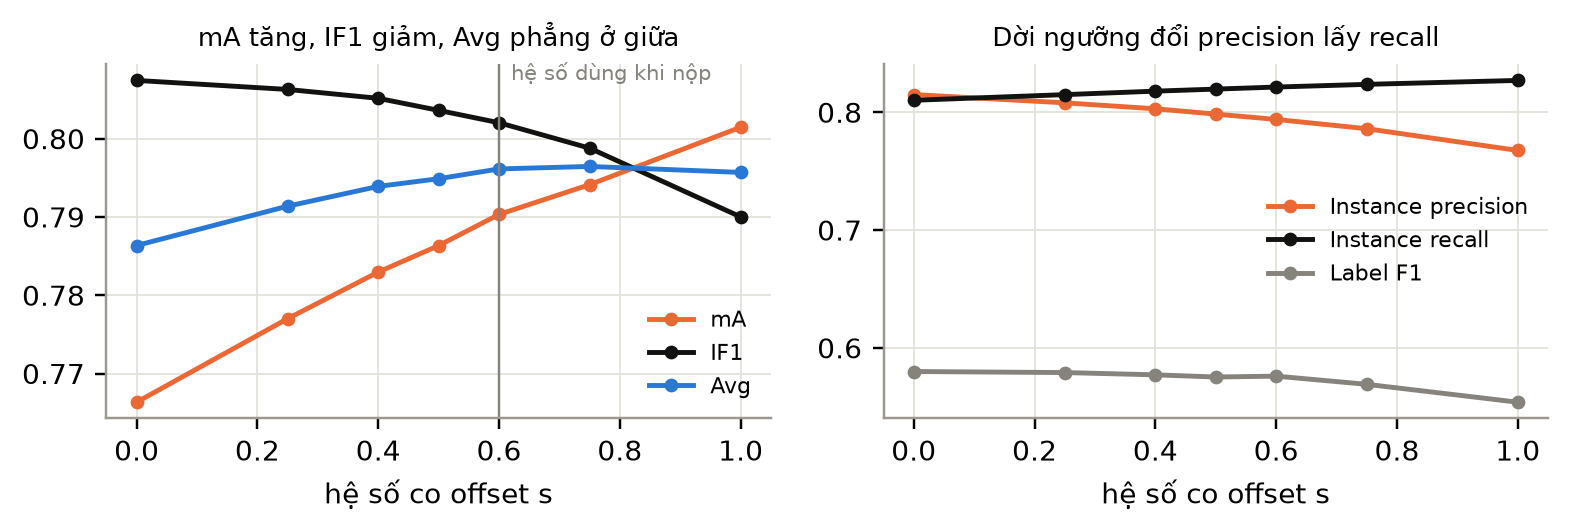
\includegraphics[width=\linewidth]{v2_metric_tradeoff.png}
\caption{Ảnh hưởng của hệ số offset lên các cách chấm, đo trên ảnh PETA. Bên trái, mA tăng, Instance F1 giảm, và điểm tổng (Avg) gần như phẳng từ 0.6 đến 1. Bên phải, dời ngưỡng làm chương trình trả lời có nhiều hơn, nên ít bỏ sót hơn (recall tăng) nhưng sai nhiều hơn (precision giảm).}
\label{fig:metric}
\end{figure}

\begin{ghichu}
Điểm tổng là sự thoả hiệp giữa hai mong muốn trái ngược, gồm nhận ra thuộc tính hiếm và không trả lời thừa. Dời ngưỡng chỉ chọn được vị trí trên đường thoả hiệp đó. Muốn cả hai cách đếm cùng tăng, chương trình phải phân biệt ảnh tốt hơn.
\end{ghichu}

\section{Chương trình của đội}
\label{sec:system}

Chương trình có hai phần. Phần thứ nhất là backbone (tạm dịch: mạng trích xuất đặc trưng). Phần này nhìn ảnh và biến nó thành một tập con số mô tả nội dung ảnh, gọi là feature (tạm dịch: đặc trưng). Đội dùng DINOv3, một mạng do Meta công bố, đã được pretrain (tạm dịch: huấn luyện sẵn) trên 1,7 tỉ ảnh thông thường. Nhờ vậy nó đã biết nhận ra hình dạng, màu sắc và chất liệu trước khi học bài toán này. DINOv3 có kiến trúc ViT (Vision Transformer, tạm dịch: mạng Transformer cho ảnh). ViT chia ảnh thành các ô vuông 16×16 pixel gọi là patch (tạm dịch: mảnh ảnh), rồi tính một feature cho mỗi patch. Đội dùng hai cỡ là ViT-B (base, khoảng 86 triệu tham số) và ViT-L (large, khoảng 300 triệu tham số).

Phần thứ hai là head (tạm dịch: phần đầu ra), biến feature thành 40 xác suất. Phiên bản đầu dùng head đơn giản nhất, cộng trung bình feature của mọi patch thành một vector chung cho cả 40 thuộc tính. Cách này có nhược điểm là thuộc tính ``đội mũ'' cũng phải dùng thông tin từ chân và từ nền phía sau người. Phiên bản sau dùng query head (tạm dịch: đầu ra truy vấn). Mỗi thuộc tính có một vector truy vấn riêng, là một dãy số được học cùng chương trình. Nhờ cơ chế attention (tạm dịch: cơ chế chú ý), vector này tự gán trọng số cao cho những patch liên quan, ví dụ vector của thuộc tính đội mũ gán trọng số cao cho các patch ở phần đầu.

Trong lúc học, chương trình so xác suất nó dự đoán với nhãn thật bằng một loss (tạm dịch: hàm đo sai số) rồi tự chỉnh để sai số nhỏ dần. Đội dùng binary cross-entropy (tạm dịch: entropy chéo nhị phân), loại loss khiến xác suất dự đoán khớp với tần suất thật. Thuộc tính hiếm được tăng trọng số để chương trình không bỏ qua chúng. Một lượt học qua toàn bộ dữ liệu gọi là một epoch (tạm dịch: vòng học). Sau khi học xong, chương trình được gắn offset như ở mục~\ref{sec:metrics}.

\section{Kiểm tra ý tưởng khi không có tập chấm}
\label{sec:proxy}

Đội không thấy ảnh chấm và chỉ được nộp ba lần mỗi ngày, nên không thể thử từng ý tưởng bằng cách nộp bài. Điểm trên ảnh cùng loại với ảnh đã học cũng không đáng tin, như con số 0.885 so với 0.777 ở trên. Đội dùng một proxy (tạm dịch: phép thử thay thế) bắt chước tình huống thật. Chương trình chỉ được học từ Market1501 và PA100k, rồi được chấm trên PETA mà nó chưa từng thấy. Nếu một ý tưởng giúp chương trình làm tốt trên PETA, có cơ sở để hy vọng nó cũng giúp trên tập chấm thật.

Mỗi lần chạy cho điểm hơi khác nhau do yếu tố ngẫu nhiên. Hai lần chạy y hệt nhau cho 0.7961 và 0.7956. Vì vậy đội chỉ giữ một ý tưởng khi nó hơn mốc so sánh ít nhất 0.003, lớn hơn nhiều so với mức dao động này.

\section{Chương trình mất điểm ở đâu}
\label{sec:analysis}

Trên PETA, chương trình có thể mất điểm vì hai lý do khác nhau. Lý do thứ nhất là nó không phân biệt được ảnh, ví dụ cho người mặc áo đỏ và người mặc áo cam xác suất ``áo đỏ'' gần bằng nhau. Lý do thứ hai là nó phân biệt đúng nhưng mọi xác suất bị lệch đều lên hoặc xuống, nên ngưỡng nằm sai chỗ. Khả năng phân biệt được đo bằng AUC (tạm dịch: diện tích dưới đường cong, đo khả năng xếp người có thuộc tính lên trên người không có). AUC không phụ thuộc vào ngưỡng.

Để tách hai lý do, đội làm một phép thử. Đội tính offset trực tiếp trên nhãn thật của PETA, gọi là oracle offset (tạm dịch: offset biết trước đáp án). Offset này không dùng được khi nộp bài vì không có nhãn của tập chấm. Nhưng nó cho biết điểm sẽ đạt bao nhiêu nếu ngưỡng được đặt đúng, và phần chênh lệch chính là phần điểm mất do ngưỡng.

\begin{figure}[H]
\centering
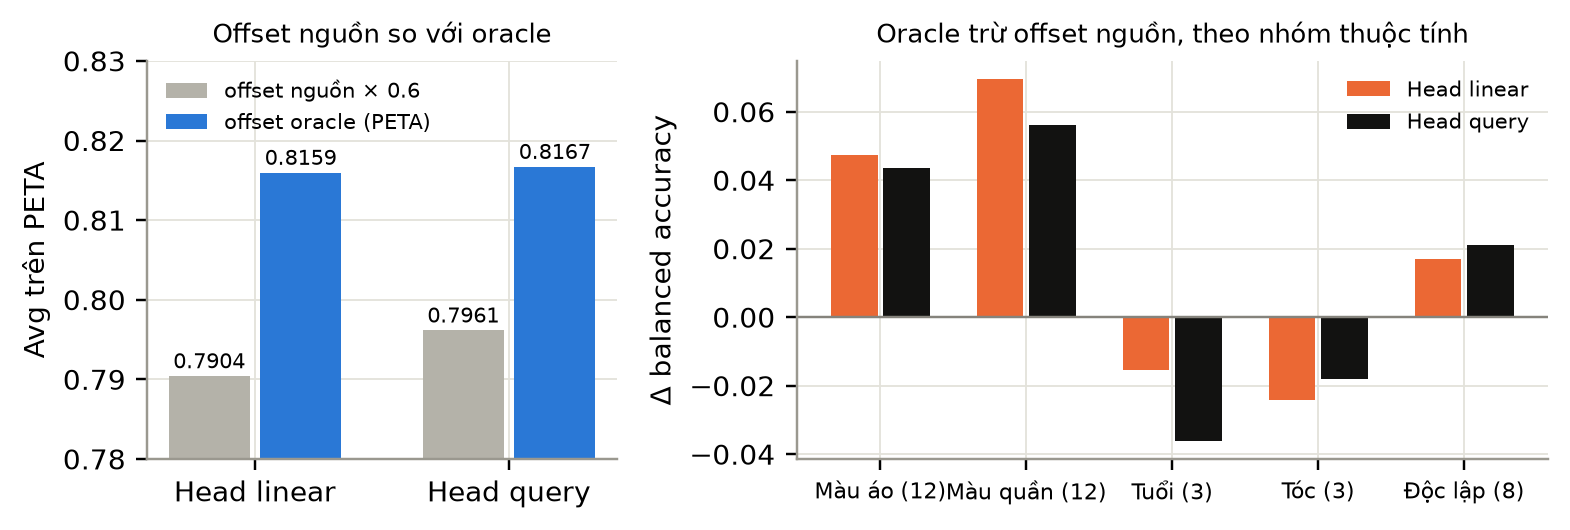
\includegraphics[width=\linewidth]{v2_gap.png}
\caption{Bên trái, điểm trên PETA khi dùng offset tính từ dữ liệu cũ và khi dùng oracle offset. Khoảng cách khoảng 0.02 là phần điểm mất do ngưỡng. Bên phải, phần mất này tập trung ở hai nhóm màu áo và màu quần.}
\label{fig:gap}
\end{figure}

Phần điểm mất do ngưỡng là khoảng 0.02 (Hình~\ref{fig:gap}), tập trung ở các thuộc tính màu. Đội đã thử giả thuyết rằng camera mới làm màu ảnh lệch đi, bằng cách cho chương trình học với ảnh bị đổi màu ngẫu nhiên, nhưng lỗi không giảm. Giải thích phù hợp hơn là khác biệt trong cách gán nhãn màu, như việc PETA đôi khi ghi hai màu cho một chiếc áo. Nếu đúng vậy, phần lỗi này không sửa được, vì muốn biết thói quen gán nhãn của tập chấm thì phải xem nhãn của nó, và luật thi cấm việc này.

\section{Những gì đã thử}
\label{sec:sweep}

Đội thử khoảng 35 thay đổi trên proxy, chia thành bốn nhóm. Nhóm thứ nhất thay đổi head, ví dụ head nhiều lớp hơn, MoE (Mixture of Experts, tạm dịch: hỗn hợp chuyên gia, nhiều head nhỏ được chọn tuỳ ảnh), hay head xét các thuộc tính lần lượt theo thứ tự. Nhóm thứ hai thay đổi loss và cách học. Nhóm thứ ba thay đổi cách biến đổi ảnh khi học, gọi là data augmentation (tạm dịch: tăng cường dữ liệu), ví dụ lật ảnh hay đổi màu. Nhóm thứ tư thay đổi backbone và kích thước ảnh.

\begin{figure}[H]
\centering
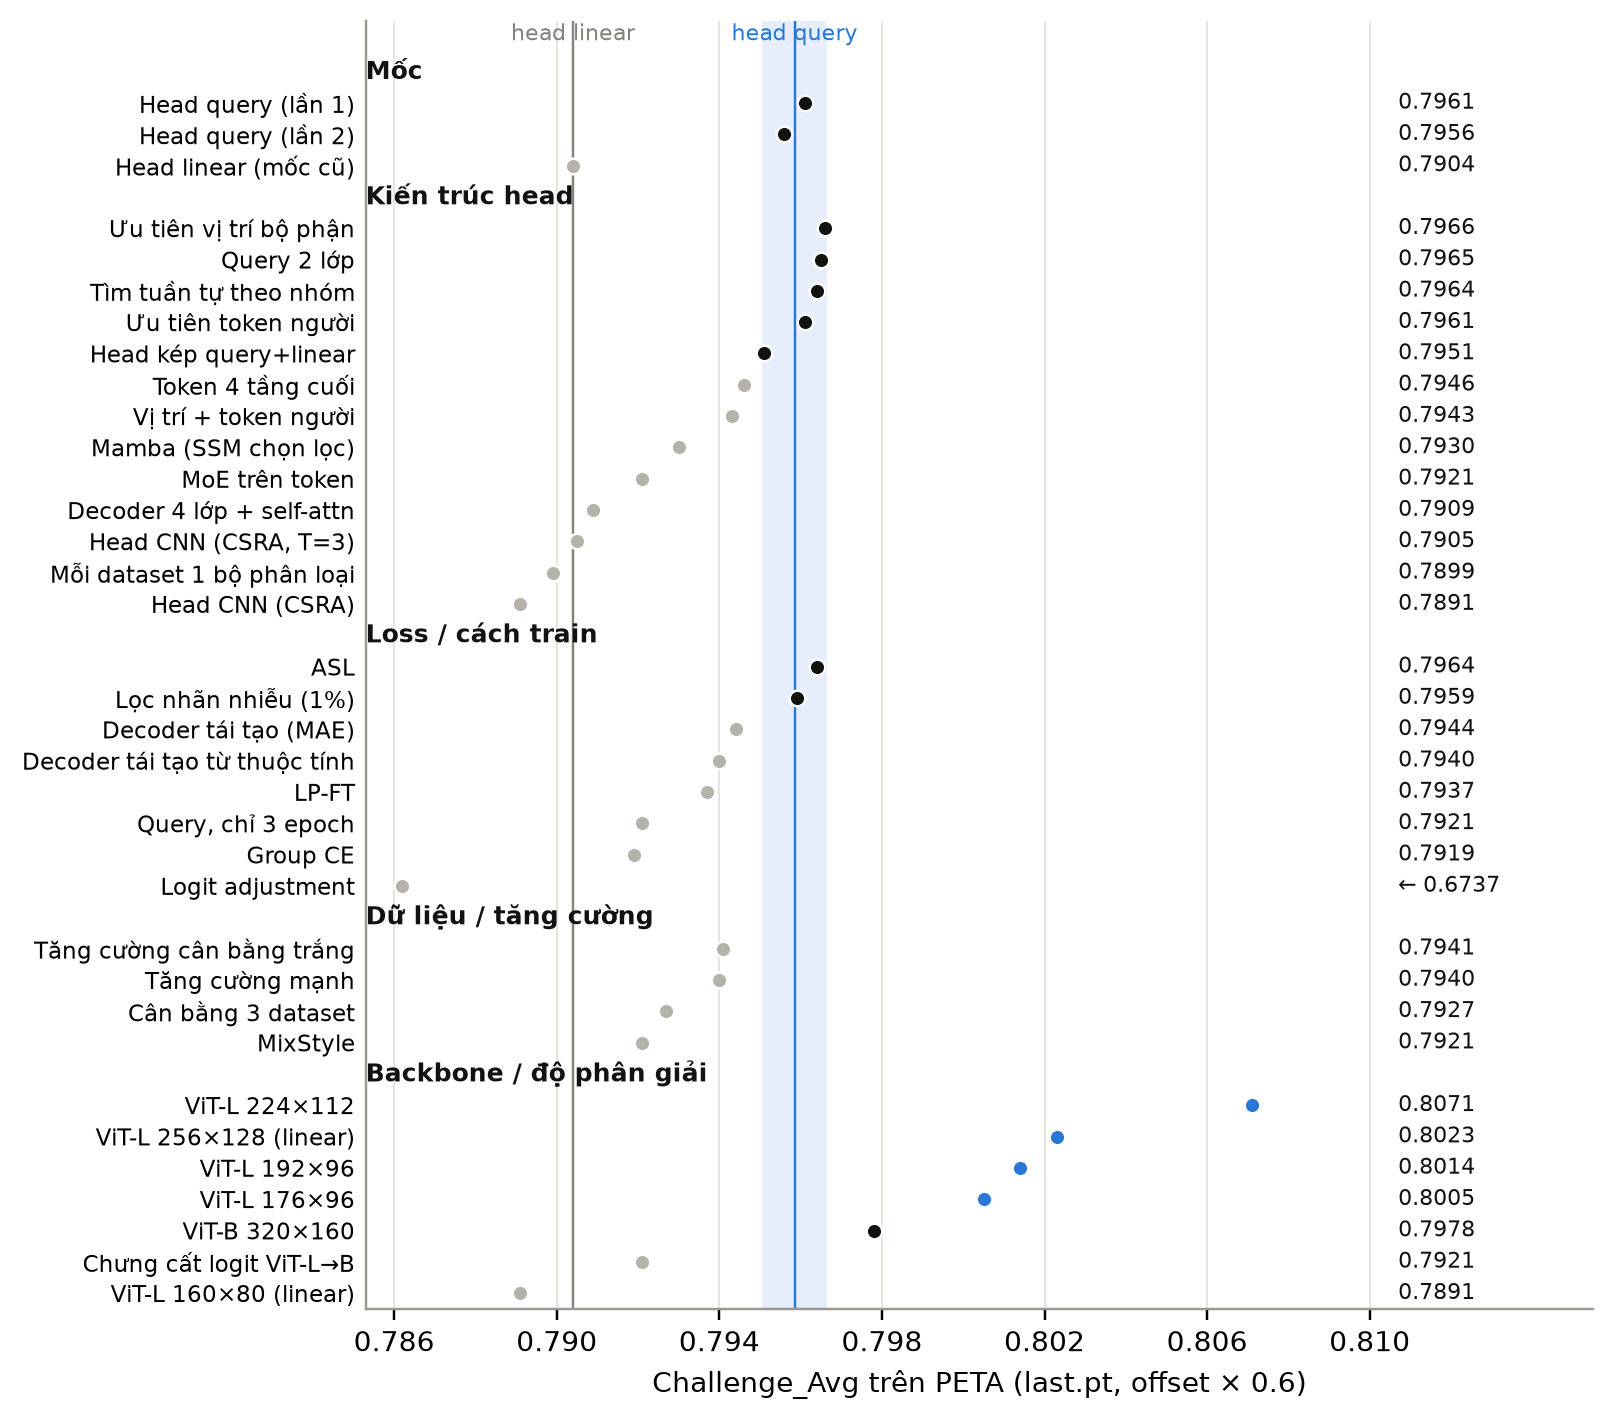
\includegraphics[width=0.82\linewidth]{v2_experiments.png}
\caption{Điểm trên proxy PETA của khoảng 35 thay đổi. Dải xanh là mốc so sánh cộng trừ mức dao động ngẫu nhiên. Chỉ những thay đổi dùng ViT-L (điểm xanh) vượt mốc rõ ràng.}
\label{fig:sweep}
\end{figure}

Hình~\ref{fig:sweep} cho thấy mọi thay đổi ở head, loss và tăng cường dữ liệu đều nằm quanh mốc hoặc thấp hơn. Head phức tạp hơn thậm chí còn kém hơn. Lý do là mọi head đều đọc cùng một bộ feature do ViT-B tạo ra. Nếu bộ feature không đủ thông tin để phân biệt hai ảnh, không head nào phân biệt được. AUC của mọi biến thể dùng ViT-B nằm trong khoảng 0.898 đến 0.908, còn ViT-L đạt 0.910 đến 0.913. Chỉ việc thay backbone bằng ViT-L làm điểm vượt mốc.

\section{Mô hình lớn hơn và giới hạn thời gian}
\label{sec:vitl}

ViT-L chính xác hơn nhưng chậm hơn khoảng 3,5 lần ViT-B. Ở kích thước ảnh 256×128 pixel, nó cần gần 2 giờ cho toàn bộ tập chấm, vượt xa giới hạn 60 phút. Đội thử quantization (tạm dịch: lượng tử hoá, lưu các con số với độ chính xác thấp hơn để tính nhanh hơn). Cách này làm ViT-L nhanh gần gấp đôi nhưng điểm giảm 0.044, nên bị loại. Cách còn lại là cho ViT-L xem ảnh nhỏ hơn. Ảnh nhỏ hơn có ít patch hơn, nên tính nhanh hơn.

Để ước lượng thời gian trên server, đội đo tốc độ trong một môi trường giống hệt server trên máy cá nhân, rồi quy đổi theo tỉ lệ đo được từ một bài nộp thật. Hình~\ref{fig:vitl} so sánh các lựa chọn. ViT-L ở 224×112 pixel đạt điểm proxy cao nhất nhưng cần khoảng 73 phút. ViT-L ở 176×96 pixel cần khoảng 48 phút và vẫn hơn ViT-B rõ rệt, nên được chọn để nộp.

\begin{figure}[H]
\centering
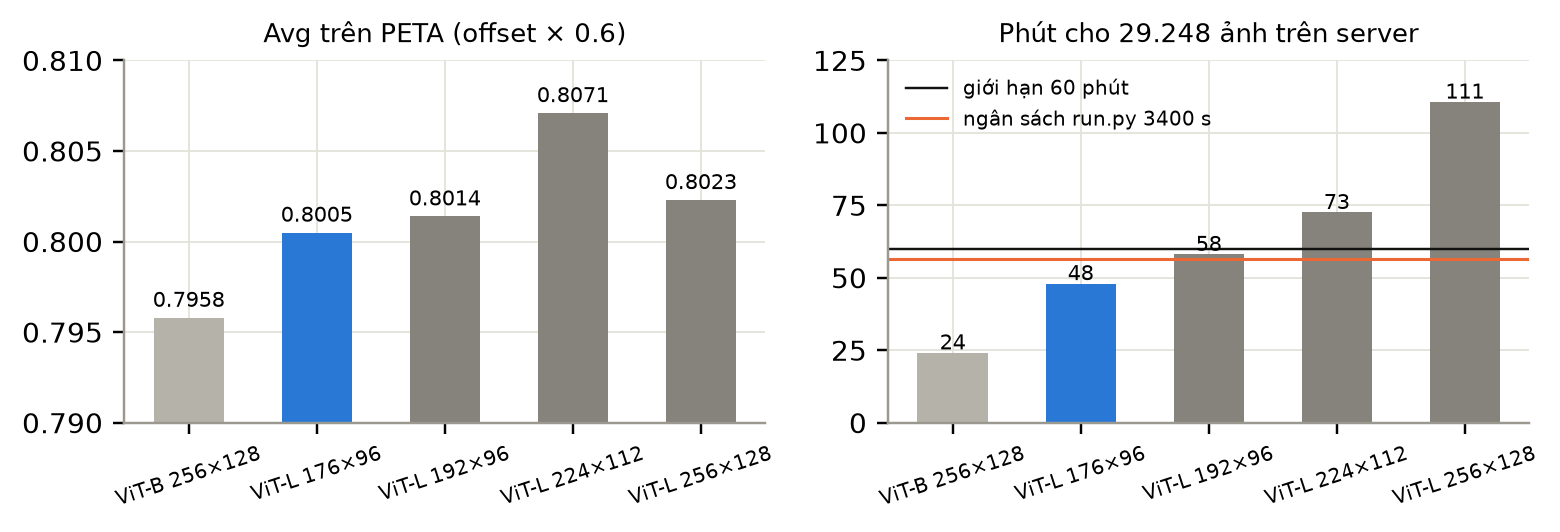
\includegraphics[width=\linewidth]{v2_vitl.png}
\caption{Bên trái, điểm proxy của ViT-B và ViT-L ở nhiều kích thước ảnh. Bên phải, thời gian ước lượng để chạy hết tập chấm trên server, so với giới hạn 60 phút. Cột xanh là lựa chọn được nộp, lựa chọn ViT-L duy nhất kịp giờ.}
\label{fig:vitl}
\end{figure}

Đội cũng đặt một giới hạn an toàn trong chương trình. Nếu đến phút thứ 57 vẫn chưa xong, chương trình trả về xác suất trung bình cho những ảnh còn lại thay vì để server dừng giữa chừng. Bài nộp vì vậy luôn có kết quả, chỉ bị mất một ít điểm ở các ảnh cuối nếu server chậm hơn dự kiến.

\section{Kết quả trên tập chấm thật}
\label{sec:test}

\begin{table}[H]
\centering\small
\begin{tabularx}{\linewidth}{@{}Xcc@{}}
\toprule
Bài nộp & Điểm proxy (PETA) & Điểm chấm thật \\
\midrule
ViT-B, head đơn giản & 0.7904 & 0.7775 \\
ViT-B, head đơn giản, offset hệ số 1 thay vì 0.6 & 0.7921 & 0.7766 \\
ViT-B, query head & 0.7958 & 0.7750 \\
ViT-L ở 176×96, query head, học từ phần train & 0.8005 & 0.7857 \\
ViT-L ở 176×96, query head, học từ cả train và val & 0.8005 & 0.7838 \\
\bottomrule
\end{tabularx}
\caption{Điểm proxy và điểm chấm thật của các bài nộp chính. Chỉ việc đổi sang ViT-L làm điểm chấm thật tăng.}
\label{tab:subs}
\end{table}

Bảng~\ref{tab:subs} cho thấy ViT-L nâng điểm chấm thật từ 0.7775 lên 0.7857, đúng như proxy dự đoán. Tuy nhiên proxy đoán sai hai lần. Query head trên ViT-B hơn head đơn giản 0.0054 trên proxy nhưng kém 0.0025 trên tập chấm thật. Offset hệ số 1 cũng hơn trên proxy nhưng kém trên tập chấm thật.

\begin{figure}[H]
\centering
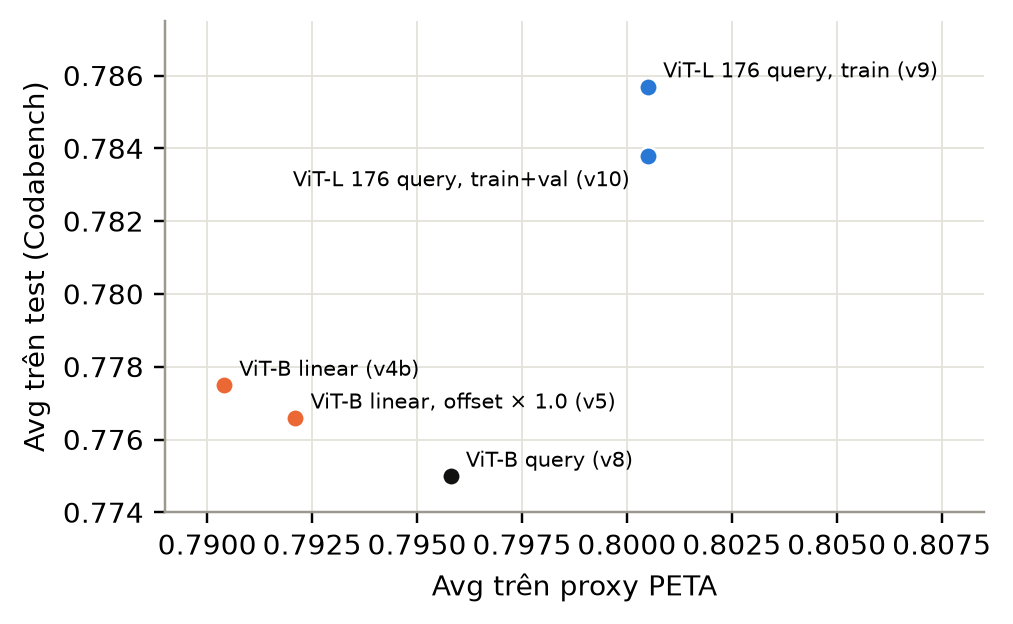
\includegraphics[width=0.52\linewidth]{v2_proxy_test.png}
\caption{Điểm proxy (trục ngang) so với điểm chấm thật (trục dọc). Đổi sang ViT-L làm cả hai cùng tăng. Hai thay đổi về ngưỡng tăng trên proxy nhưng giảm trên tập chấm thật.}
\label{fig:pt}
\end{figure}

Cả hai lần proxy đoán sai đều là thay đổi chủ yếu làm ngưỡng khớp hơn với PETA. Mục~\ref{sec:analysis} đã cho thấy ngưỡng phụ thuộc vào thói quen gán nhãn của từng bộ dữ liệu, nên khớp với PETA không có nghĩa là khớp với tập chấm. Ngược lại, ViT-L làm tăng AUC. Nó xếp người có thuộc tính lên trên người không có chính xác hơn, và khả năng này không phụ thuộc vào ngưỡng hay thói quen gán nhãn. Vì thế mức tăng của nó chuyển được sang tập chấm thật.

\begin{ghichu}
Proxy dùng một bộ dữ liệu chỉ đáng tin với những thay đổi giúp chương trình phân biệt ảnh tốt hơn, thể hiện qua AUC tăng. Một thay đổi chỉ làm điểm proxy tăng mà AUC không tăng nhiều khả năng chỉ khớp với thói quen gán nhãn của PETA.
\end{ghichu}

\section{Việc tiếp theo}

\paragraph{Ngay lập tức.} Bảng xếp hạng đang giữ bài nộp gần nhất (0.7838). Đội nên nộp lại bài 0.7857 để nó thành bài gần nhất.

\paragraph{Dùng sức mạnh của ViT-L mà vẫn kịp giờ.} Đây là hướng duy nhất đã cho kết quả thật. Có ba cách. Cách thứ nhất là cho ViT-B học bắt chước feature của ViT-L, gọi là distillation (tạm dịch: chưng cất kiến thức). Lần thử trước chỉ bắt chước xác suất đầu ra nên không hiệu quả. Cách thứ hai là gộp các patch giống nhau, ví dụ các patch nền, để ViT-L tính ít hơn. Cách thứ ba là bỏ bớt vài lớp cuối của ViT-L.

\paragraph{Làm phép thử đáng tin hơn.} Thêm hai proxy giữ lại Market1501 và PA100k, chạy lặp mỗi thí nghiệm nhiều lần, và chỉ giữ thay đổi làm tăng AUC trên mọi proxy.

\paragraph{Giới hạn của báo cáo.} Mức dao động ngẫu nhiên mới được ước lượng từ hai lần chạy. Giả thuyết về thói quen gán nhãn chưa được kiểm chứng trực tiếp. Tỉ lệ quy đổi thời gian giữa máy cá nhân và server dựa trên một lần đo.

\end{document}
